\documentclass[a4paper]{article}

\usepackage[danish]{babel}
\usepackage[utf8]{inputenc}
\usepackage[T1]{fontenc}
\usepackage{graphicx}

\title{FTM-1}

\begin{document}

\maketitle

% \begin{comment}
%   Outline:
%   - instruktioner - og at flytte data
%   - registrene X,Y,Z,W
%   - instruktionsformat
%   - "instruktioner med tal i": registeret K
%   - at regne: R og C
%   - hukommelsen
%   - hvor kommer instruktioner fra?: registeret IP
%   - at ændre i hukommelsen
%   - I/O - et output-device: tal-printeren.
%         - et input-device: tilfældigheds-generatoren?
%   - at tage beslutninger
%   - Subrutiner
%
%   Gennemgående:
%   - Maskin-cyklussen
%   - Opgaver
% \end{comment}

\section*{Forord}
Dette er et forsøg på at lave en computer-model, som er velegnet til at demonstrere og undervise i computeres basale virkemåde.

Modellen hedder ``FTM-1'' -- for ``Fra-Til-Maskine nummer 1''.
Der er nemlig kun én type instruktion: at kopiere data fra ét sted til et andet.
I en forstand kan modellen altså ikke blive simplere.

Samtidig er det et mål med modellen, at den skal være fleksibel nok til kunne at dække output i f.eks. billed- og lyd-format, så den kan skalere op til rigtige spil.
\medskip

Der er mange lag i computere -- fra fysik over elektronik og bit til
tal, repræsentationer af tekst, billeder og lyd, op til programmer og
systemer.
Denne model starter ved tal og arbejder opad. Bits og det binære
talsystem springes altså helt over: maskinen er baseret på decimal-tal.

\newpage

\section{Instruktioner}


\subsection*{Hvad kan en computer?}
Nogle vigtige dele af, hvad en computer kan, er:

\begin{itemize}\setlength\itemsep{0pt}
\item Flytte rundt på data
\item Lave beregninger
\item Tage beslutninger
\item Få data fra verden
\item Styre ting -- f.eks. motorer og skærme
\end{itemize}

De tre første ting er noget, der sker inde i maskinen.
De sidste to ting handler om at computeren gør nogte med omverdenen --
det, der kaldes \emph{input} og \emph{output}: input fra verden til
computeren og output fra computeren til verden.

Vi skal nok nå at se på alle disse ting -- men vi starter med den
første: at flytte rundt på data.

\subsection*{Hvad er data?}
``Data'' kan være mange ting -- et billede, en lyd, et program, et tal, et bogstav, et ord, en liste af ord, en video\ldots
Men alle disse ting kan bygges op af tal. Så det, maskinen arbejder med, er tal: 0, 1, 2, 3\ldots{} og $-1$, $-2$, $-3$\ldots

\subsection*{At flytte data}

Den computer, vi skal lege med, hedder FTM-1 (for ``Fra-Til-Maskine'').
I FTM-1 er der et antal \emph{steder}, hvor der bor tal.
Stederne har \emph{navne} og \emph{indhold}.
Indholdet -- de tal, der bor alle stederne -- ikke de samme hele
tiden; de ændrer sig hele tiden.
Men stedernes navne ændrer sig ikke. Dem kan du se på figur \ref{ftm1-arch} -- de er de hvide rektangler.
Nogle af stederne er specielle. Men dem venter vi lidt med.

\begin{figure}
  \label{ftm1-arch}
  \centering
  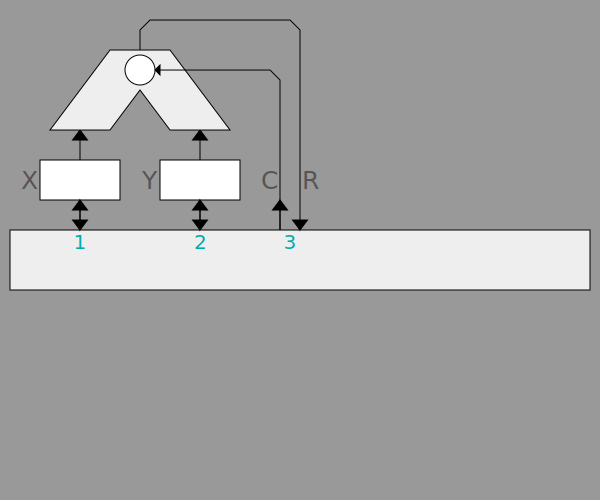
\includegraphics[width=10cm]{cpu}
  \caption{Diagram over FTM-1.}
\end{figure}

Maskinen FTM-1 kan én ting: at flytte -- eller mere præcist: kopiere
-- data fra ét sted til et andet.

\subsection*{Instruktioner}

En \emph{instruktion} er en besked om, hvad man skal gøre.
En computer gør ikke andet end at følge sådan nogle beskeder.
De beskeder, en computer kan forstå, er meget simple -- men til
gengæld kan computeren udføre dem rigtig hurtigt. Nogle kan gøre over
en milliard ting i sekundet. Selv om det er meget simple ting, er en
milliard rigtig meget. Så meget, at man kan få computere til at gøre
meget indviklede ting.

\subsection*{FTM-1's instruktioner}
Den maskine, vi skal bruge -- FTM-1 -- har kun én slags instruktion:
man kan bede den om at flytte data.
I instruktionen står der, hvor data skal flyttes fra og til. Det er
derfor, maskinen hedder en ``Fra-Til-Maskine''.

Man kan skrive instruktioner.
Sådan en instruktion skrives med en pil fra navnet på ``fra''-stedet til navnet på ``til''-stedet -- sådan her:

$$X \to Y$$

\noindent
eller med tegnet \texttt{>}, der er lettere at skrive på en computer:

$$\texttt{X>Y}$$

\subsection*{Udførelse af  instruktioner}
Når computeren udfører en instruktion, sker det i to skridt:
\begin{enumerate}\setlength\itemsep{0pt}
\item Læs en værdi (et tal) fra ``fra''-stedet
\item Skriv den samme værdi til ``til''-stedet
\end{enumerate}

Vi starter med kun at se på stederne X, Y, Z og W.
Hvis nu de steder starter med at indeholde disse tal:

\begin{center}
\begin{tabular}{lrrrr}
Navn: & X & Y & Z & W\\
\hline
Indhold: & 12 & 34 & 56 & 789\\
\end{tabular}
\end{center}

\noindent
og maskinen så udfører instruktionen
$$X \to Y$$

\noindent
så vil maskinen læse værdien \emph{12} fra X, og skrive den i Y, så
værdierne bagefter er:

\begin{center}
\begin{tabular}{lrrrr}
Navn: & X & Y & Z & W\\
\hline
Indhold: & 12 & 12 & 56 & 789\\
\end{tabular}
\end{center}

\subsection*{Opgaver}
\begin{enumerate}
\item Hvis X=12, Y=34, Z=56 og W=789 før en instruktion, hvad bliver
  indholdet så af de fire steder, hvis instruktionen er
  \begin{enumerate}
  \item $Y \to X$ ?
  \item $W \to Y$ ?
  \item $X \to W$ ?
  \end{enumerate}

\item Hvis X=12, Y=34, Z=56 og W=789 før en instruktion, hvad er de så
  bagefter, hvis maskinen udfører instruktionerne $X \to Y$ og
  $W \to X$, i dén rækkefølge?

%\item Kan du bytte om på værdien af X og Y (så X kommer til at
%  indeholde 34 og Y kommer til at indeholde 12),

\item Hvis vi starter med X=12, Y=34, Z=56 og W=789, hvilke af disse
  situationer kan du så komme frem til med én eller flere
  instruktioner, hvor du kun må bruge de fire steder?

  \begin{center}
    \begin{tabular}{lrrrr}
      & X & Y & Z & W\\
      \hline
      Indhold før: & 12 & 34 & 56 & 789\\
      \hline
      Indhold efter:\\
      Situation a) & 12 & 12 & 12 & 12\\
      Situation b) & 789 & 789 & 34 & 34\\
      Situation c) & 12 & 34 & 100 & 56\\
      Situation d) & 34 & 12 & 56 & 789\\
      Situation e) & 34 & 12 & 56 & 56\\
    \end{tabular}
  \end{center}
  Hvad kan lade sig gøre, og hvad kan ikke?
  %Hvordan kan man komme frem til den situation? (Eller: hvorfor kan man ikke?)

\end{enumerate}

\newpage
\section{Instruktioner kan skrives som tal}
% Om indkodning af instruktioner som tal.

\section{Instruktioner med tal i}
% Om registeret "K".

\section{Beregninger}
% Om ALU'en og registerparret "R"/"C".

\section{Hvor kommer instruktionerne fra?}
% Om hukommelse og registeret IP - "instruktionspegeren".
% Om at hoppe.
% Om at stoppe maskinen (IP<0).

\section{Hukommelsen}
% Om at læse fra og skrive til hukommelsen.

\section{Input og output}

\section{Beslutninger}
% Om registeret "J".
% Om sammenlignings-operatorer, og sandt/falsk.
% Evt. om brug af ALU-operation 0 & 1.
% Evt. i omvendt rækkefølge - "J" til sidst?

\section{Subrutiner}
% Om registeret "L".

\end{document}
